\section{Tracibility and Correctness of Implementation}~\label{sec:correct}

\todo{Discuss the implementation of labels, ACSL contracts, and proofs}

The SBV backend generates one function per expression of the reified AST (abstract syntax tree). Thus the main task consists in generating a contract for the expression, which can be done by induction on the syntax. This is very similar to writing a pretty printer for expressions (corresponding to the token $\langle funStream \rangle$ in the grammar), except for some tricks, which have to be taken into account, which are often due to the absence of implementation of some features described in ACSL.

\begin{itemize}
	\item No let bindings can be written in ACSL contracts.
	\subitem It was decided to do not support let bindings during ACSL contract generation, thus making a code containing let bindings unprovable. Nevertheless, the programmer can use a functional style, changing the let bindings into function, at the cost of having arguments in order to use variables that should be in scope for let bindings.
	\item No mathematical functions are available (sin, cos, tan, sqrt, ...).
	\subitem This is quite normal, given that on embedded systems, the access to math.h is not guaranteed. Thus we decided to transform each trigonometrical function into a call to an external function, called the same way (or sinf if working on floats), and it's up to the user to provide an implementation of the function (or to choose the standard implementation in math.h).
	\item No global invariants are implemented in WP plugin.
	\subitem We split the dereferencing of the pointer in an external function (called ident, which is equivalent to the identity), which allows to have simple enough contracts to be able to prove the assertions, and given that the splitting does not change the semantics of the program (it is similar to an beta-expansion).
	\item No bitwise operator.
	\subitem SBV library was changed in that purpose, and bitwise operators have been deprecated\footnote{https://github.com/LeventErkok/sbv/issues/177}.
\end{itemize}

As requested by the DO-178B norm regarding the safety of critical flight avionics, a traceability has to be ensured between the origin haskell source code file and the generated C code produced. For that purpose, a labeling system was implemented, similar to the trace instruction from Debug.Trace, but prints its label in the C source file instead of stdout. Moreover, the fact that the expressions could be huge after reification (all functions are beta expanded in expressions), it caused problems with frama-c which could not parse contracts of 500000 characters long. 

For this purpose, three features were implemented. 
\begin{itemize}
	\item The first is a prover mode, which will optimize the code in order to make it easier to prove (by splitting absolute values in half for example).
	\item The second is a pretty printer of the AST into a dot file, which then generates a graph of what a C file is supposed to do (this graph is equivalent to the ACSL contract, so it is easier to see a problem in the contract by looking at the AST graph).
	\item The last are magic characters in labels, which can affect the generated C code when the compilation is in mode prover. The only one implemented is the character \texttt{?} which causes the backend to cut the AST at this node and create an other one. This is done by using the identity as external function which is shown in the Figure~\ref{fig:splitting label} for the following simple Copilot code :
\end{itemize} 
\begin{lstlisting}[frame=single,language=haskell]
	import qualified Copilot.Compile.SBV as S
	
	alt :: Stream Bool
	alt = (label "?splitting" $ not $ externB "externvar" Nothing)
	
	spec :: Spec
	spec = do
	trigger "trigger" (alt) []
	
	main = do
	reify spec >>= S.proofACSL S.defaultParams
\end{lstlisting}
\begin{figure}[!htb]
	\vspace*{2cm}
	\includegraphics[width=42mm]{images/label/main.ps}
	\includegraphics[width=42mm]{images/label/splitted.ps}
	\includegraphics[width=42mm]{images/label/splitted2.ps}
	\caption{The splitting process. The AST on the left is split into two smaller ASTs, that then generate two separate functions into two separate files, making it easier to prove the contracts for them.}
	\label{fig:splitting label}
\end{figure}
